\documentclass{beamer}
\usepackage{animate}
\usepackage{multimedia}
\usepackage[english,russian]{babel}

\usepackage{pgfpages}
\setbeameroption{show notes on second screen}
%https://tug.ctan.org/macros/latex/contrib/beamer/doc/beameruserguide.pdf

\usepackage[T2A]{fontenc}
\usepackage[utf8]{inputenc}

\setbeamertemplate{caption}[numbered]

\usetheme{CambridgeUS}
\usecolortheme{dolphin}


\title[Сплайны]{Поверхности}
\author[Быковских Д.А.]{Быковских Дмитрий Александрович}
\date{18.11.2023}

\begin{document}
	\begin{frame}
		\titlepage
	\end{frame}

	\begin{frame}{Введение}
		Традиционный способ построения/представления объемной модели с помощью  ортогональной проекции.

		Ортогональная проекция --- сеть ортогональных кривых, используемых для изображения трехмерных объектов на плоскости.
		
		Такую модель удобно исследовать с целью получения различных \textquotedbl физических\textquotedbl~ характеристик: размер, объем, площадь поверхности, угол кривизны и др.

		Причины
		\begin{itemize}
			\item Создание объемных моделей с нуля в соответствии с концептуальными и дизайнерскими требованиями.
			\item Реконструкция трехмерной модели может потребоваться на основе данных, полученных из сканирования реальных объектов (медицина);
		\end{itemize}

		\note{
			\begin{figure} 
				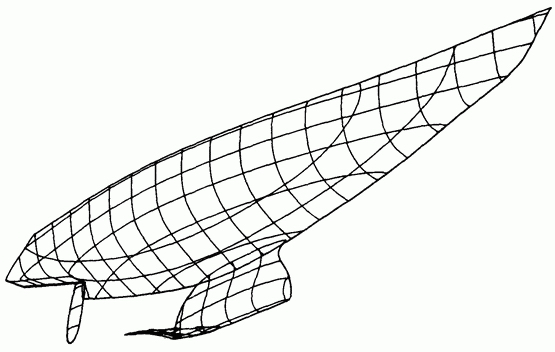
\includegraphics[width=0.61\textwidth]{images/airship-model.jpg}
				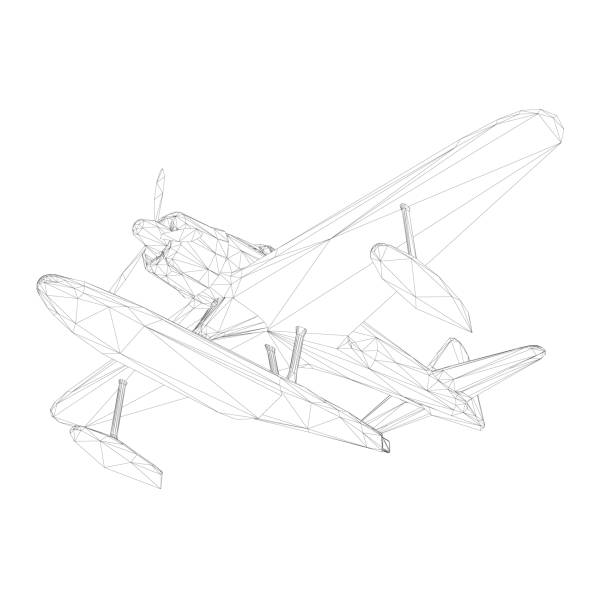
\includegraphics[width=0.38\textwidth]{images/airplane-model.jpg}
				\caption{Каркасные модели}
			\end{figure}
		}

	\end{frame}	


	\begin{frame}{Отображение параметрических поверхностей}

		Поверхность удобнее отображать из параметрического двумерного пространства $uv$ в трехмерное объективное пространство $xyz$.

		Параметры $(u,v) \to (x,y,z)$, где $u,v \in [0,1]$.

		Пример
		\[
		\begin{cases}
			x(u,v) = 3u +v \\
			y(u,v) = 2u +3v +uv \\
			z(u,v) = 0 \\
		\end{cases}	
		\]

		\note{
			\begin{figure} 
				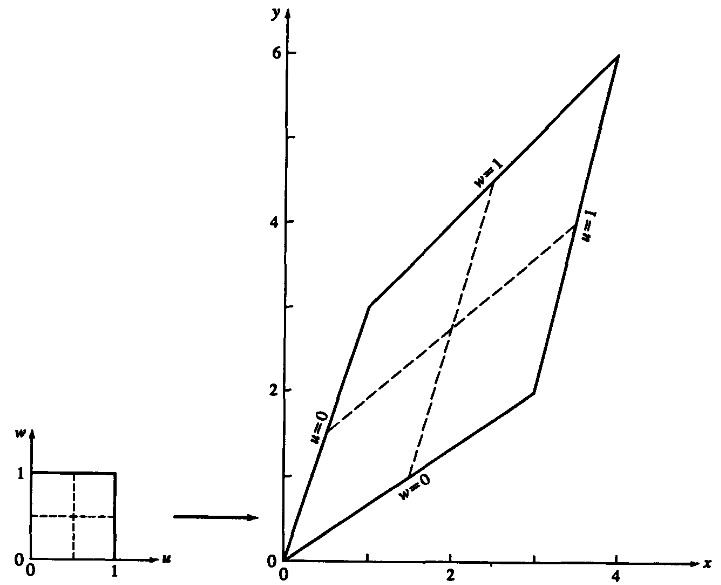
\includegraphics[width=0.65\textwidth]{images/example1.png}
				\caption{Параметрическое пространство (слева) и объектное пространство (справа)}
			\end{figure}
		}

	\end{frame}

	\begin{frame}{Билинейная поверхность}
		
		Билинейная поверхность конструируется из 4х угловых точек:
		$P(0,0)$, $P(1,0)$, $P(0,1)$, $P(1,1)$.
		
		Любая точка поверхности $S(u,v)$ определяется линейной интерполяцией между противоположными границами единичного квадрата.

		\[
			S(u,v) = 
			\begin{bmatrix}
				1-u \\
				u \\
			\end{bmatrix}^T
			\begin{bmatrix}
				P(0,0) & P(0,1) \\
				P(1,0) & P(1,1) \\
			\end{bmatrix}
			\begin{bmatrix}
				1-v \\
				v \\
			\end{bmatrix}
			,
		\]
		где $u,v \in [0,1]$.

		
		\note{
			\[
				S(u,v) = 
				P(0,0)(1-u)(1-v)
				+
				P(0,1)(1-u)v
				+
				P(1,0)u(1-v)
				+
				P(1,1)uv
			\]
			Примечание. \\
			Легко проверить, подставив значения в параметры $u, v$.

			При этом координаты точек $P$ можно задавать произвольным образом.
		}

	\end{frame}

	\begin{frame}{Билинейная поверхность}{Пример}
		Задача. \\ Найти т. $P(0.5,0.5)$ билинейной поверхности, заданной координатами: \\
		$P(0,0)=[0~0~1]$,
		$P(0,1)=[1~1~1]$,
		$P(1,0)=[1~0~0]$,
		$P(1,1)=[0~1~0]$.

		Решение:
		\[
			S(u,v) =
			\begin{cases}
				x(u,v) = (1-u)v + u(1-v) \\
				y(u,v) = (1-u)v + uv \\
				z(u,v) = (1-u)(1-v) + (1-u)v \\
			\end{cases}
		\]

		Ответ:
		\[
			P(0.5,0.5) = [0.5~0.5~0.5]
			\]

			\note{
				\begin{figure} 
					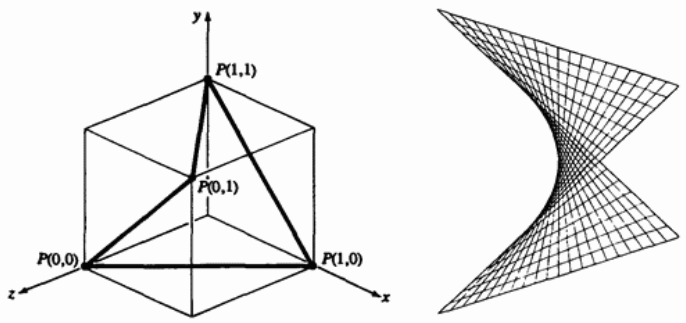
\includegraphics[width=\textwidth]{images/example2.png}
					\caption{Билинейная поверхность. Определяющие угловые точки (слева). поверхность (справа)}
				\end{figure}
			}


	\end{frame}

	\begin{frame}{Линейчатые поверхности}
		Линейчатая поверхность --- поверхность, образованная движением прямой линии.
		\\ Прямые, принадлежащие этой поверхности, называются прямолинейными образующими.  \\
		Каждая кривая, пересекающая все прямолинейные образующие, называется направляющей кривой.

		Линейчатая поверхность образуется при движении прямой линии вдоль направляющей с одной стороны степенью свободы.
		\begin{itemize}
			\item 
			Линейчатые поверхности: \\
			плоскость, конусы, цилиндры.
			\item
			Двулинейчатые поверхности: \\
			однополостный гиперболоид, гиперболический параболоид.
		\end{itemize}




			Такие поверхности важны в промышленности, при построении техники.

			\note{
				\begin{figure} 
					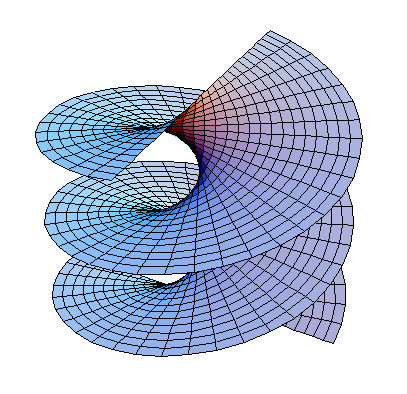
\includegraphics[width=0.51\textwidth]{images/Helicoid.png}
					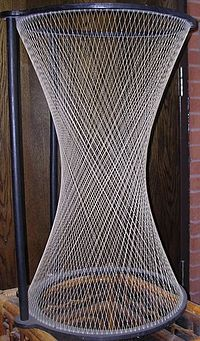
\includegraphics[width=0.29\textwidth]{images/hyperboloid.jpg}
					\caption{Геликоид (слева) и однополостный гиперболоид (справа)}
				\end{figure}
			}

		\end{frame}

		\begin{frame}{Линейчатые поверхности}

			\[
				S(u,v) = 
				\begin{bmatrix}
					1-v \\
					v \\
				\end{bmatrix}^T
				\begin{bmatrix}
					P(u,0) \\
					P(u,1) \\
				\end{bmatrix}
				=
				P(u,0)(1-v)+P(u,1)v
				,
				\]
				где $P(u,0)=f(u)$, $P(u,1)=g(u)$.

				\[
					S(u,v) = 
					\begin{bmatrix}
						1-u \\
						u \\
					\end{bmatrix}^T
					\begin{bmatrix}
						P(0,v) \\
						P(1,v) \\
					\end{bmatrix}
					=
					P(0,v)(1-u)+P(1,v)u
					,
				\]
				где $P(0,v)=f(v)$, $P(1,v)=g(v)$.
			\end{frame}

			\begin{frame}{Однополостный гиперболоид, цилиндр, конус}{Пример}
				
				\[
					S(u,v) = 
					\begin{bmatrix}
						1-v \\
						v \\
					\end{bmatrix}^T
					\begin{bmatrix}
						P(u,0) \\
						P(u,1) \\
					\end{bmatrix}
					=
					P(u,0)(1-v)+P(u,1)v
					,
					\]
					где \\ $P(u,0)=
					[
						\cos (u-\varphi)~
						\sin (u-\varphi)~
						-1
					]$, $P(u,1)=[
						\cos(u+\varphi)~
						\sin(u+\varphi)~
						1
					]$.

					В основе лежат две окружности (направляющие). \\
					В зависимости от дополнительного параметра $\varphi$ получаются следующие типы поверхностей:
					\begin{itemize}
						\item 
						при $ \varphi=0 $ получается цилиндр $x^2+y^2=1$;
						\item
						при $ \varphi=\pi/2 $ получается конус $x^2+y^2=z^2$;
						\item
						при $ 0<\varphi<\pi/2 $ получается однополостный гиперболоид $\tfrac{x^2}{a^2}+\tfrac{y^2}{a^2}-\tfrac{z^2}{c^2}=1$, где $ \ a=\cos\varphi\;,\; c=\cot \varphi$.
					\end{itemize}


			\note{
				\begin{figure} 
					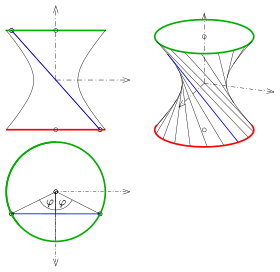
\includegraphics[width=0.5\textwidth]{images/hyperboloid.png}
					\caption{Однополостный гиперболоид, где $\varphi =\pi/3$}
				\end{figure}
			}
		\end{frame}

		\begin{frame}{Бикубическая поверхность Кунса}
			В основе лежит кубическое уравнение, описывающие поведение граничной кривой
			\[
			P(t) = B_0 + B_1 t +B_2 t^2 +B_3 t^3
			,	
			\]
			где $t \in [0,1]$. 

			Каждая из четырех граничных кривых $P(u,0)$, $P(u,1)$, $P(0,v)$, $P(1,v)$ задается следующим образом:

			\[
				P(t) = [T][N][G] =
				\begin{bmatrix}
					t^3 \\
					t^2 \\
					t \\
					1 \\
				\end{bmatrix}^T
				\begin{bmatrix}
					2 & -2 & 1 & 1 \\
					-3 & 3 & -2 & -1 \\
					0 & 0 & 1 & 0 \\
					1 & 0 & 0 & 0 \\
				\end{bmatrix}
				\begin{bmatrix}
					P_0 \\
					P_1 \\
					P'_0 \\
					P'_1	\\
				\end{bmatrix}
				,
			\]
			где $t \in [0,1]$ (т.е. $t$ --- это $u$, $v$), а
			$P_0$, $P_1$, $P'_0$, $P'_1$ --- координатные и касательные векторы. 

			\note{
					Тогда смешивающие функции имеют вид:
					\[
						[F] = [T][N] =
						\begin{bmatrix}
							F_0(t) \\
							F_1(t) \\
							F_2(t) \\
							P_3(t)	\\
						\end{bmatrix}^T
						=
						\begin{bmatrix}
							t^3 \\
							t^2 \\
							t \\
							1 \\
						\end{bmatrix}^T
						\begin{bmatrix}
							2 & -2 & 1 & 1 \\
							-3 & 3 & -2 & -1 \\
							0 & 0 & 1 & 0 \\
							1 & 0 & 0 & 0 \\
						\end{bmatrix}
					\]
				}

		\end{frame}

	\begin{frame}{Бикубическая поверхность Кунса}
		\[
			S(u,v) = [U][N][P][N]^T[W]
			,
		\]
		где
		$ u =
		\begin{bmatrix}
			u^3 \\
			u^2 \\
			u \\
			1 \\
		\end{bmatrix}^T$,
		$ v =
		\begin{bmatrix}
			v^3 \\
			v^2 \\
			v \\
			1 \\
		\end{bmatrix}^T
		$.
		\[
			S(u,v) = 
			\begin{bmatrix}
				F_0(u) \\
				F_1(u) \\
				F_2(u) \\
				F_3(u) \\
			\end{bmatrix}^T
			\begin{bmatrix}
				P(0,0) & P(0,1) & P_v(0,0) & P_v(0,1) \\
				P(1,0) & P(1,1) & P_v(1,0) & P_v(1,1) \\
				P_u(0,0) & P_u(0,1) & P_{uv}(0,0) & P_{uv}(0,1) \\
				P_u(1,0) & P_u(1,1) & P_{uv}(1,0) & P_{uv}(1,1) \\
			\end{bmatrix}
			\begin{bmatrix}
				F_0(v) \\
				F_1(v) \\
				F_2(v) \\
				F_3(v) \\
			\end{bmatrix}
			,
		\]
		где $u,v \in [0,1]$.

		\[
			\begin{bmatrix}
				P
			\end{bmatrix}
			=
			\begin{bmatrix}
				\text{угловые координатные векторы} & v\text{-касательные векторы} \\
				u\text{-касательные векторы} & \text{векторы кручения} \\
			\end{bmatrix}
			\]

			\note{
				\begin{figure} 
					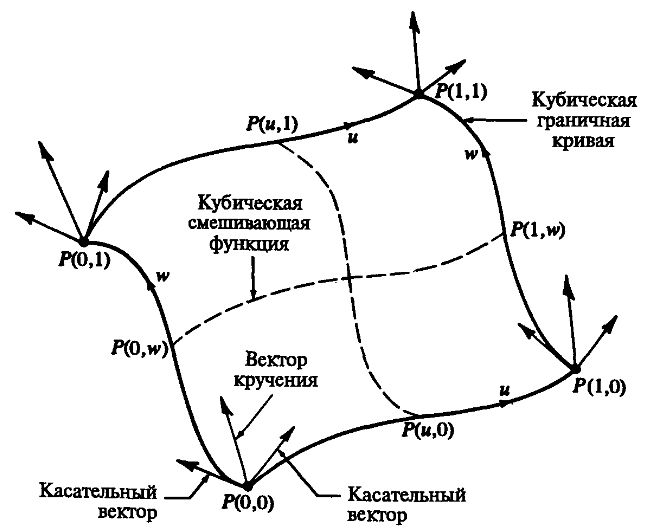
\includegraphics[width=0.65\textwidth]{images/example3.png}
					\caption{Геометрия для куска бикубической поверхности Кунса}
				\end{figure}
			}
	\end{frame}

	\begin{frame}{Поверхность Безье}
		\[
			S(u,v) = \sum_{i=0}^{n}\sum_{j=0}^{m} P_{i,j} B_{n,i}(u) K_{m,j}(v)
		,
		\]
		где глобальные базисные функции (многочлены Бернштейна) имеют вид
		\[
			B_{n,i}(u)
			=
			C_n^i u^i (1-u)^{n-i}
		\]
		\[
			K_{m,j}(v)
			=
			C_m^j v^j (1-v)^{m-j}
		\]

		\note{
			\begin{figure} 
				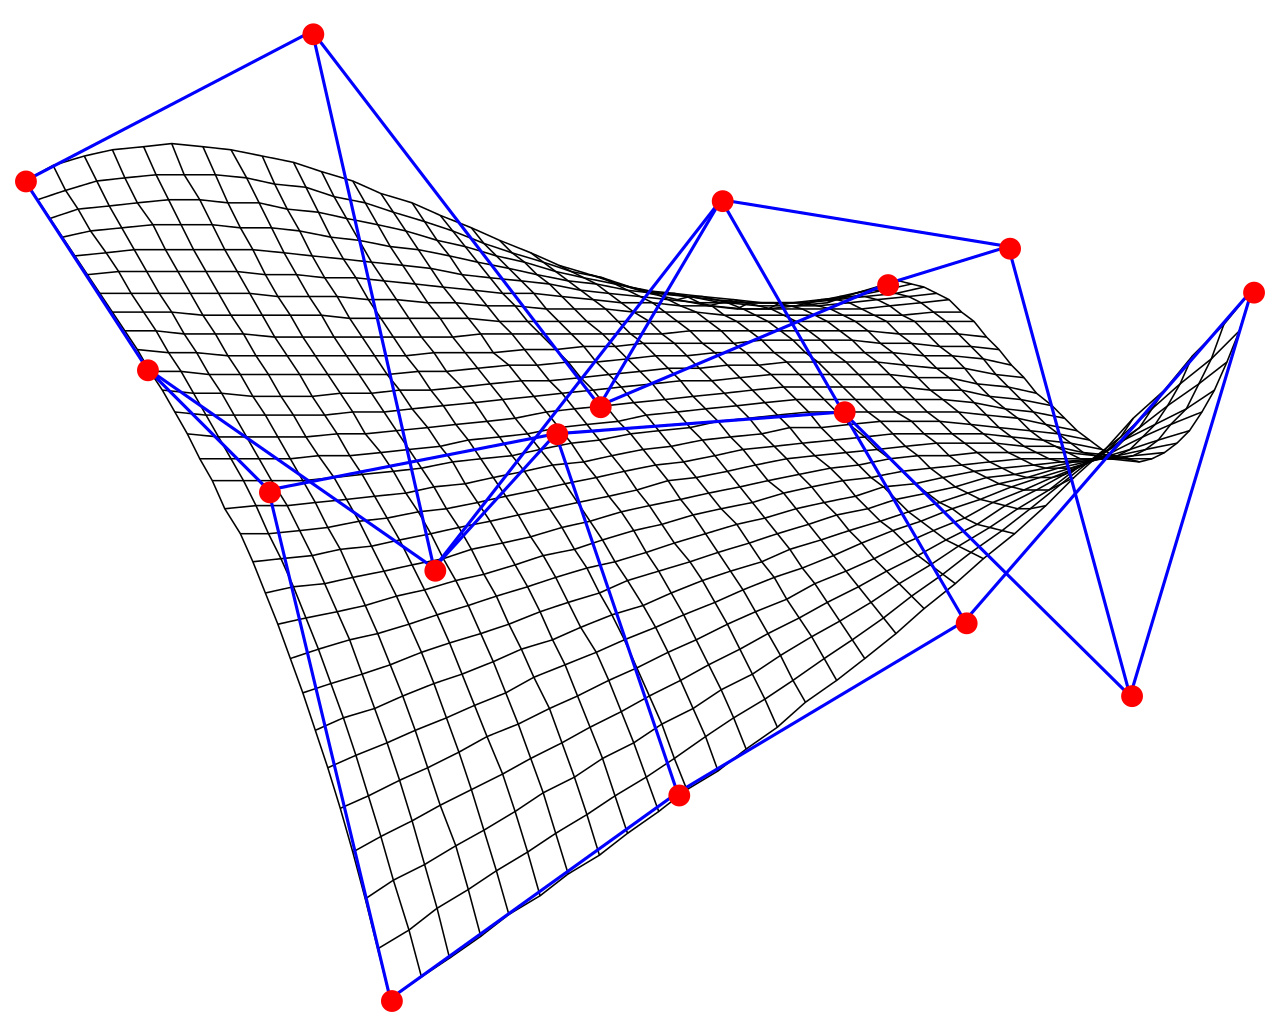
\includegraphics[width=0.45\textwidth]{images/Bezier_surface.png}
				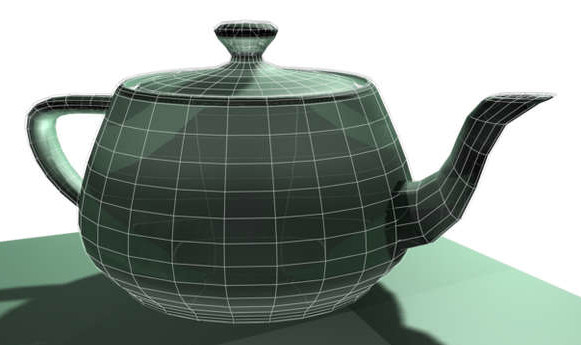
\includegraphics[width=0.45\textwidth]{images/utah_teapot.jpg}
				\caption{Поверхность Безье: модель при $n=m=3$(слева), чайник из Юты(справа)}
			\end{figure}
		}
	\end{frame}

	\begin{frame}{B-сплайн поверхность}
		\[
			S(u,v) = \sum_{i=0}^{n}\sum_{j=0}^{m} P_{i,j} N_{i,k}(u) K_{j,l}(v)
		,
		\]
		где $N_{i,k}(u) K_{j,l}(v)$ локальные базисные функции, основанные на рекуррентных формулах Кокса-де Бура.

		\note{
			\begin{figure} 
				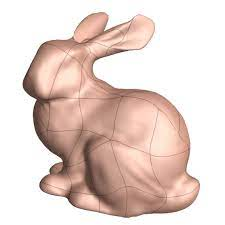
\includegraphics[width=0.5\textwidth]{images/b-spline_surface.jpg}
				\caption{B-сплайн поверхность}
			\end{figure}
		}

	\end{frame}

	\end{document}

	\[
		\begin{bmatrix}
			1 & 0 & 0 & 0 \\
			0 & 1 & 0 & 0 \\
			0 & 0 & 1 & 0 \\
			-\frac{left + right}{2} & -\frac{bottom + top}{2} & 0 & 1 \\
		\end{bmatrix}	
	\]
	
	% https://learnwebgl.brown37.net/08_projections/projections_ortho.html
	% https://www.songho.ca/opengl/gl_projectionmatrix.html
	% https://www.scratchapixel.com/lessons/3d-basic-rendering/perspective-and-orthographic-projection-matrix/opengl-perspective-projection-matrix.html
	% https://en.wikipedia.org/wiki/Viewing_frustum
	% https://www.reddit.com/r/opengl/comments/2hs6cf/questionglmfrustum_or_glmperspective/
	% https://startandroid.ru/ru/uroki/vse-uroki-spiskom/401-urok-172-perspective-frustum-ortho.html
	% http://doc.51windows.net/Directx9_SDK/graphics/programmingguide/fixedfunction/viewportsclipping/viewingfrustum.htm
	% https://www.google.com/search?q=camera+transformation+FOV&tbm=isch&ved=2ahUKEwjh6-yX7_CBAxXwBxAIHS7gDtwQ2-cCegQIABAA&oq=camera+transformation+FOV&gs_lcp=CgNpbWcQAzoHCAAQigUQQzoFCAAQgAQ6BggAEAgQHjoHCAAQGBCABDoECAAQHlDSAlizDWDWDmgBcAB4AIABUYgBwwKSAQE2mAEAoAEBqgELZ3dzLXdpei1pbWfAAQE&sclient=img&ei=mxYoZaGyMvCPwPAPrsC74A0&bih=921&biw=1920#imgrc=1JjqcwhhFgAhiM



	\begin{figure} 
		\href{https://www.researchgate.net/figure/Outline-of-the-graphics-pipeline_fig1_281810652}{
			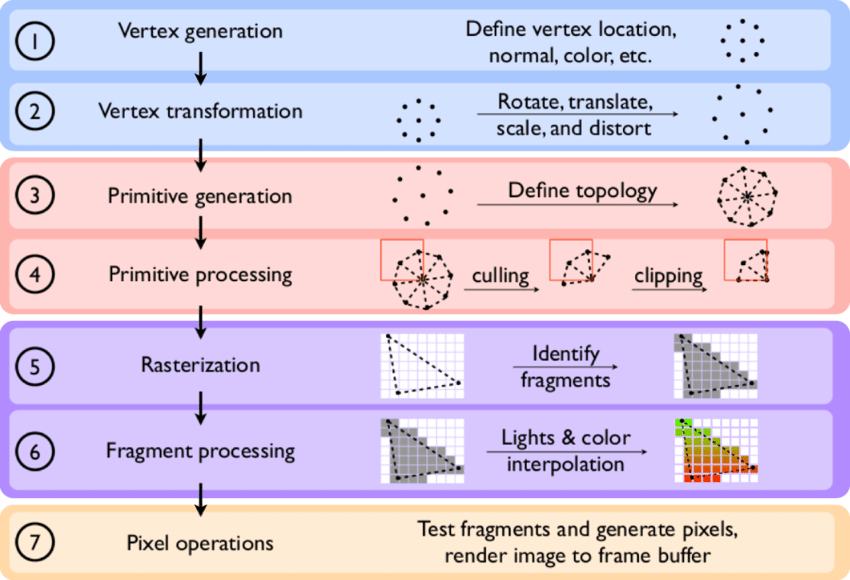
\includegraphics[width=0.75\textwidth]{images/Outline-of-the-graphics-pipeline.png}}
		\caption{Схема графического конвейера}
	\end{figure}

	\begin{figure} 
			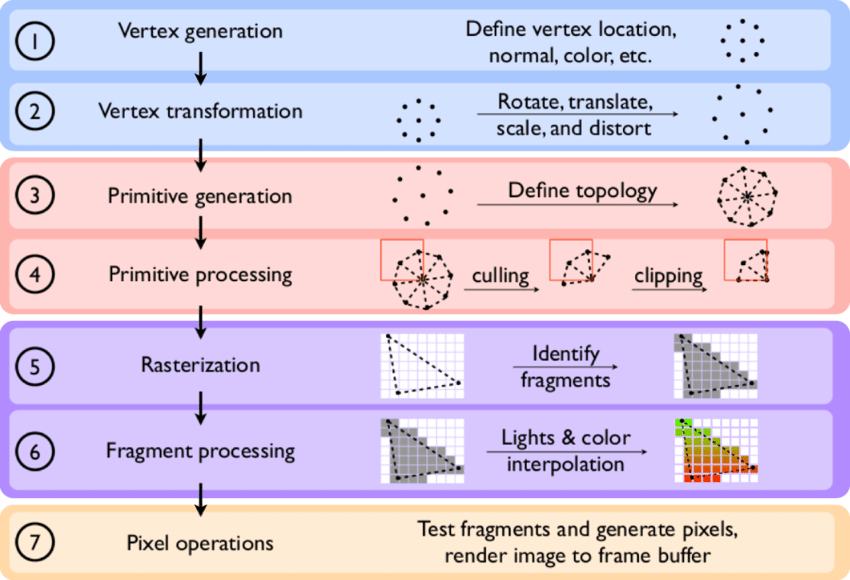
\includegraphics[width=0.75\textwidth]{images/Outline-of-the-graphics-pipeline.png}
		\caption{Схема графического конвейера}
	\end{figure}

	\begin{columns}
		\begin{column}{0.5\textwidth}
			\begin{figure} 
				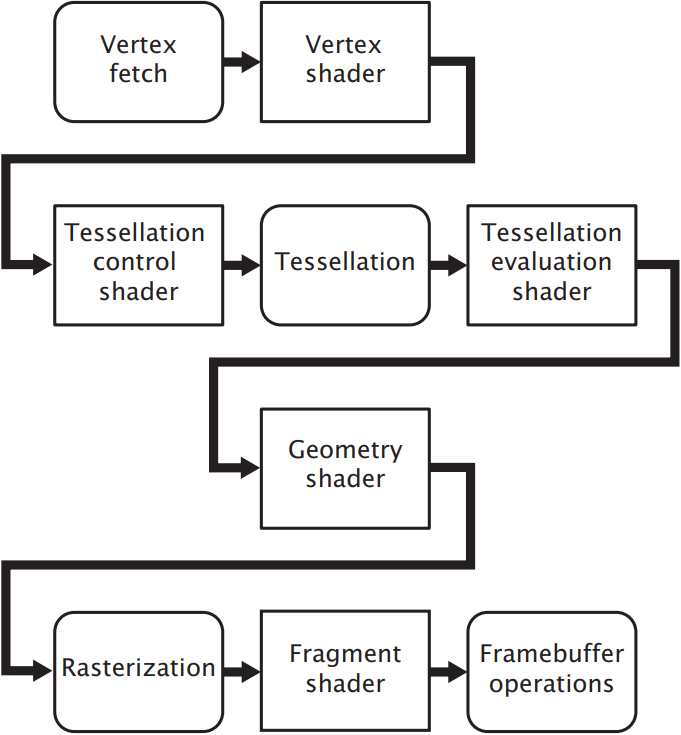
\includegraphics[width=0.9\textwidth]{images/Simplified_model_of_the_graphics_pipeline.png}
				\caption {Порядок вычисления шейдеров}
			\end{figure}
		\end{column}
		\begin{column}{0.5\textwidth}
		\end{column}
	\end{columns}
			

			\footnotesize

			\begin{table}
				% \caption{\label{tab:fractal} Название}
				\begin{center}
					\begin{tabular}{|c|c|c|}
						\hline
						$k$ & $l$ & $N(l)$ \\
						\hline
						0 & $1$ & $1$ \\
						\hline
						1 & $1/2$ & $3$ \\
						\hline
						2 & $1/4$ & $9$ \\
						\hline
						\multicolumn{3}{|c|} {\dots} \\
						\hline
						n & $2^{-n}$ & $3^{n}$ \\
						\hline
					\end{tabular}
				\end{center}
			\end{table}